\documentclass[]{beamer}
% \usepackage{beamerthemelined}
\usepackage{pstricks}
\usepackage{amsfonts,amssymb,amsmath,amsthm}
\usepackage{graphicx}
\usepackage{wallpaper}
\usepackage{color}

% \setbeamertemplate{navigation symbols}{}
\beamertemplatenavigationsymbolsempty

\usetheme{Boadilla}
\usecolortheme{whale}
\setbeamertemplate{itemize items}[triangle]


\title{Cosmic Inflation}
\author{Paho Lurie-Gregg, Michael Perlin}
\date{}

\newcommand{\f}[2]{\dfrac{#1}{#2}}
\newcommand{\p}[1]{\left(#1\right)}
\renewcommand{\t}[1]{\text{#1}}
\newcommand{\abs}[1]{\left|#1\right|}

\renewcommand{\red}[1]{{\bf \color{red} #1}}
\newcommand{\fixme}[1]{\red{[#1]}}

\begin{document}

\begin{frame}
  \maketitle
  \begin{center}
    \fixme{paper title}
    \vspace{1.5in}
  \end{center}

\end{frame}


\begin{frame}
  \frametitle{What / Why}
  sds
\end{frame}

\begin{frame}
  \frametitle{$E$ / $B$ Maps}
  \begin{figure}
    \centering
    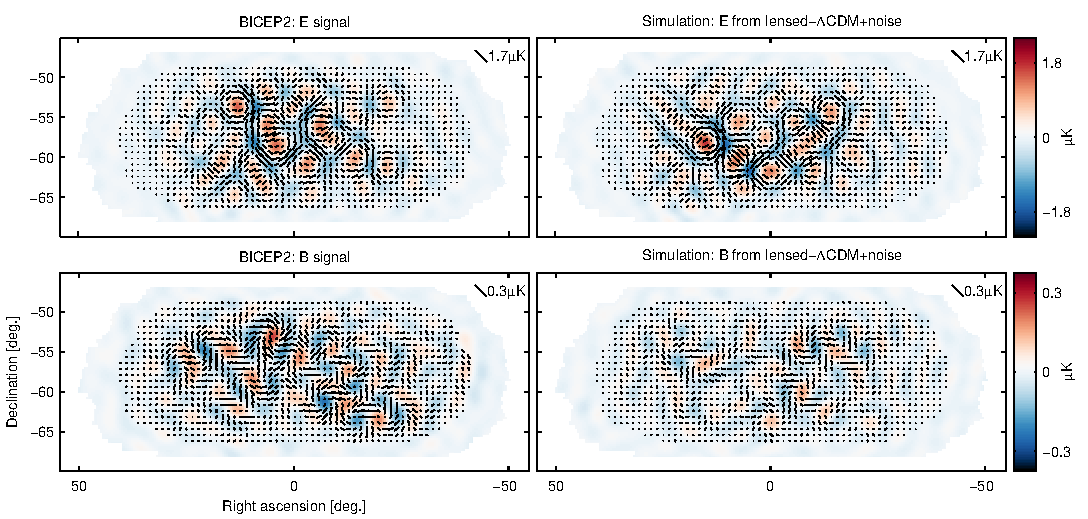
\includegraphics[width=\columnwidth]{eb_maps}
  \end{figure}
\end{frame}


\end{document}
